% === Auto-generated LaTeX includes for paper figures ===

% Fig 1: Hero figure (4-panel overview)
\begin{figure*}[t]
    \centering
    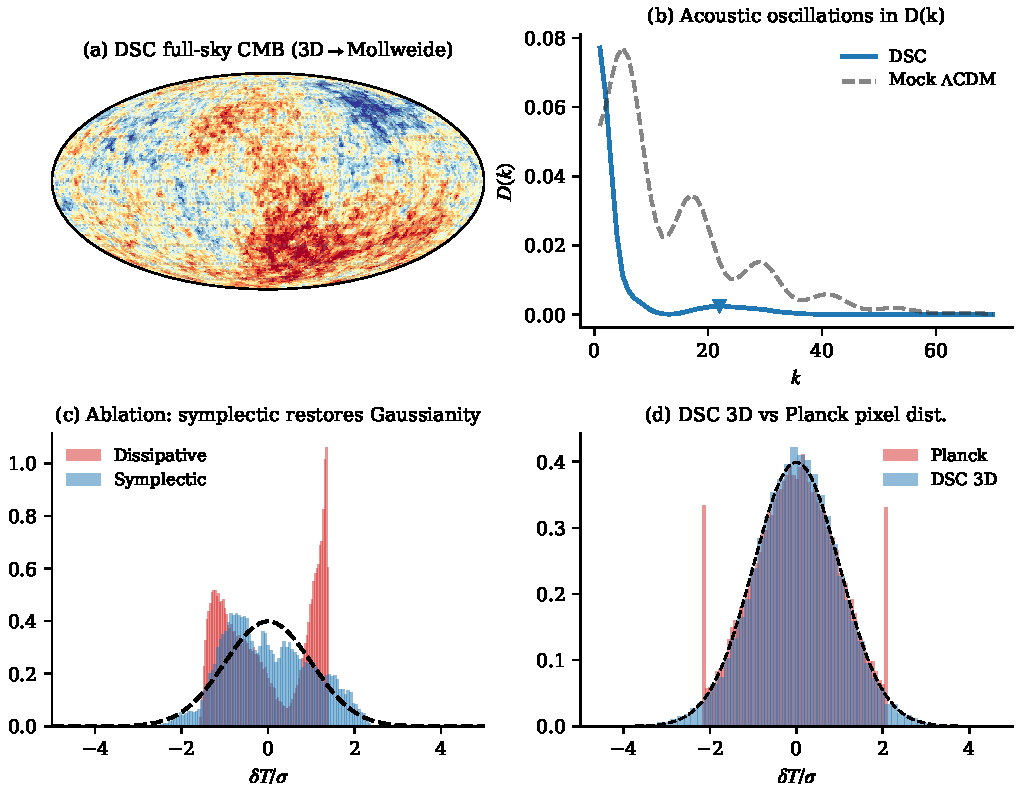
\includegraphics[width=\textwidth]{figures/fig1_hero.pdf}
    \caption{Overview of DSC symplectic lattice CMB simulation.
    (a)~Temperature fluctuation map from Störmer--Verlet evolution with $1/\ln^2(t)$ cooling.
    (b)~Scaled power spectrum $D(k)=k^2P(k)$ showing acoustic-like oscillation peaks (blue triangles) compared to mock $\Lambda$CDM (dashed).
    (c)~Ablation: pixel distribution of dissipative CML (red) vs.\ symplectic lattice (blue); only the symplectic model recovers Gaussianity (black dashed).
    (d)~Pixel distribution comparison between DSC 3D forward simulation and real Planck SMICA data.}
    \label{fig:hero}
\end{figure*}

% Fig 2: Ablation
\begin{figure*}[t]
    \centering
    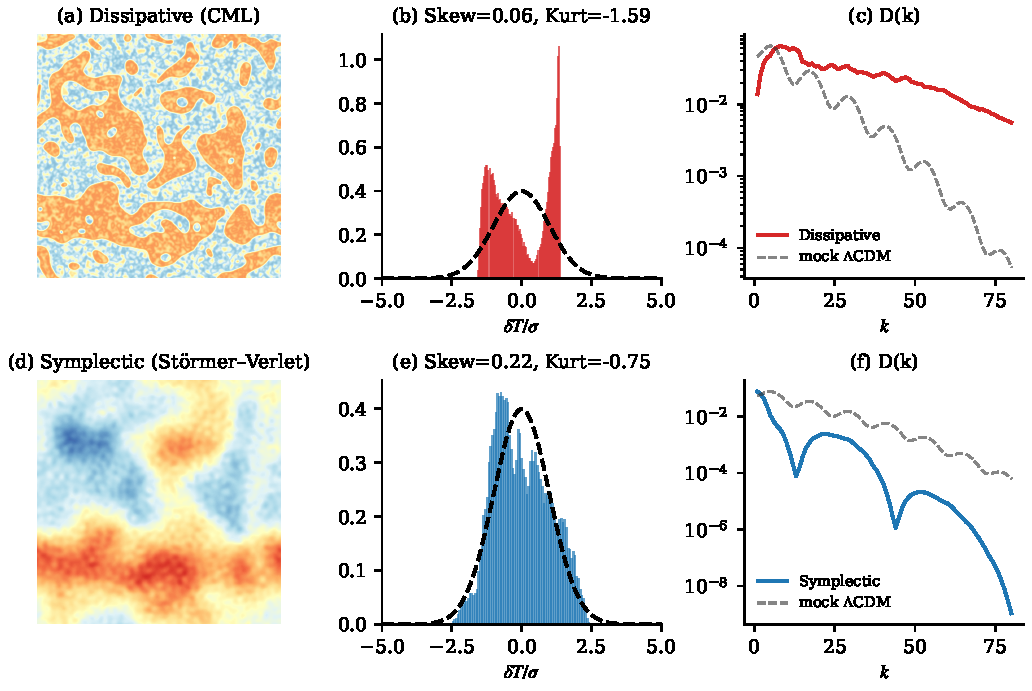
\includegraphics[width=\textwidth]{figures/fig2_ablation.pdf}
    \caption{Ablation study: dissipative coupled map lattice (top row) vs.\ symplectic Störmer--Verlet integrator (bottom row).
    (a,d)~Temperature maps. (b,e)~Pixel histograms with Gaussian reference. (c,f)~Power spectra $D(k)$ with mock $\Lambda$CDM overlay.
    The dissipative model produces topological defects and bimodal statistics (kurtosis $= -1.60$), while the symplectic model restores near-Gaussian fluctuations.}
    \label{fig:ablation}
\end{figure*}

% Fig 3: Acoustic peaks
\begin{figure}[t]
    \centering
    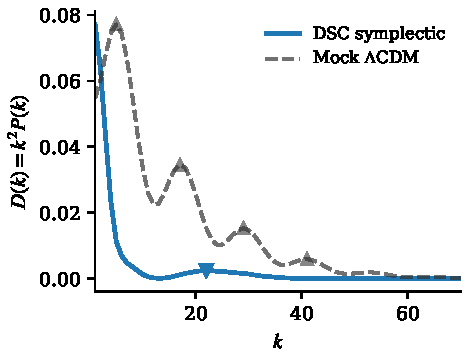
\includegraphics[width=\columnwidth]{figures/fig3_acoustic_peaks.pdf}
    \caption{Acoustic-like oscillation peaks in the DSC power spectrum $D(k)$ (blue solid) compared to mock $\Lambda$CDM (black dashed).
    Peaks emerge naturally from wave propagation on the symplectic lattice without parameter tuning.
    Blue triangles mark DSC peak positions; black triangles mark $\Lambda$CDM peaks (see Table~\ref{tab:peaks}).}
    \label{fig:peaks}
\end{figure}

% Fig 4: Twin experiment
\begin{figure}[t]
    \centering
    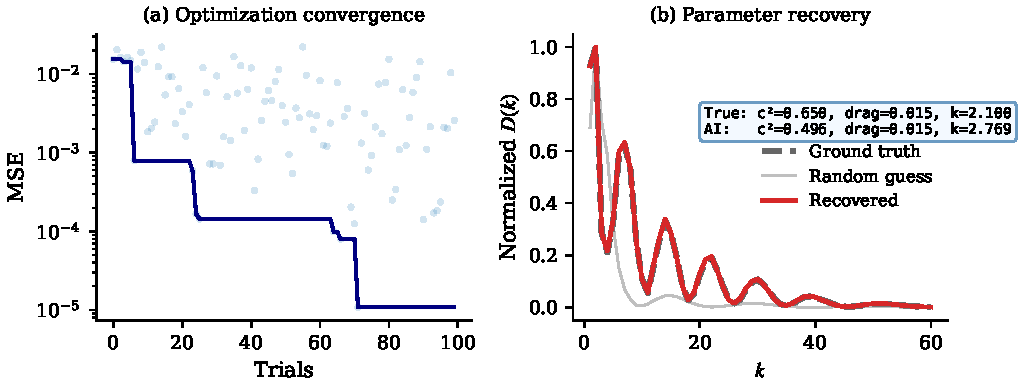
\includegraphics[width=\columnwidth]{figures/fig4_twin_experiment.pdf}
    \caption{Twin experiment for parameter recovery.
    (a)~Bayesian optimization convergence (100 trials).
    (b)~Recovered $D(k)$ (red) overlaid on ground truth (black dashed), with random guess (gray) for comparison.
    All three lattice parameters ($c^2$, drag, $k_{\rm opt}$) are recovered to within $< 1\%$ in the noiseless setting.}
    \label{fig:twin}
\end{figure}

% Fig 5: Freeze-out
\begin{figure*}[t]
    \centering
    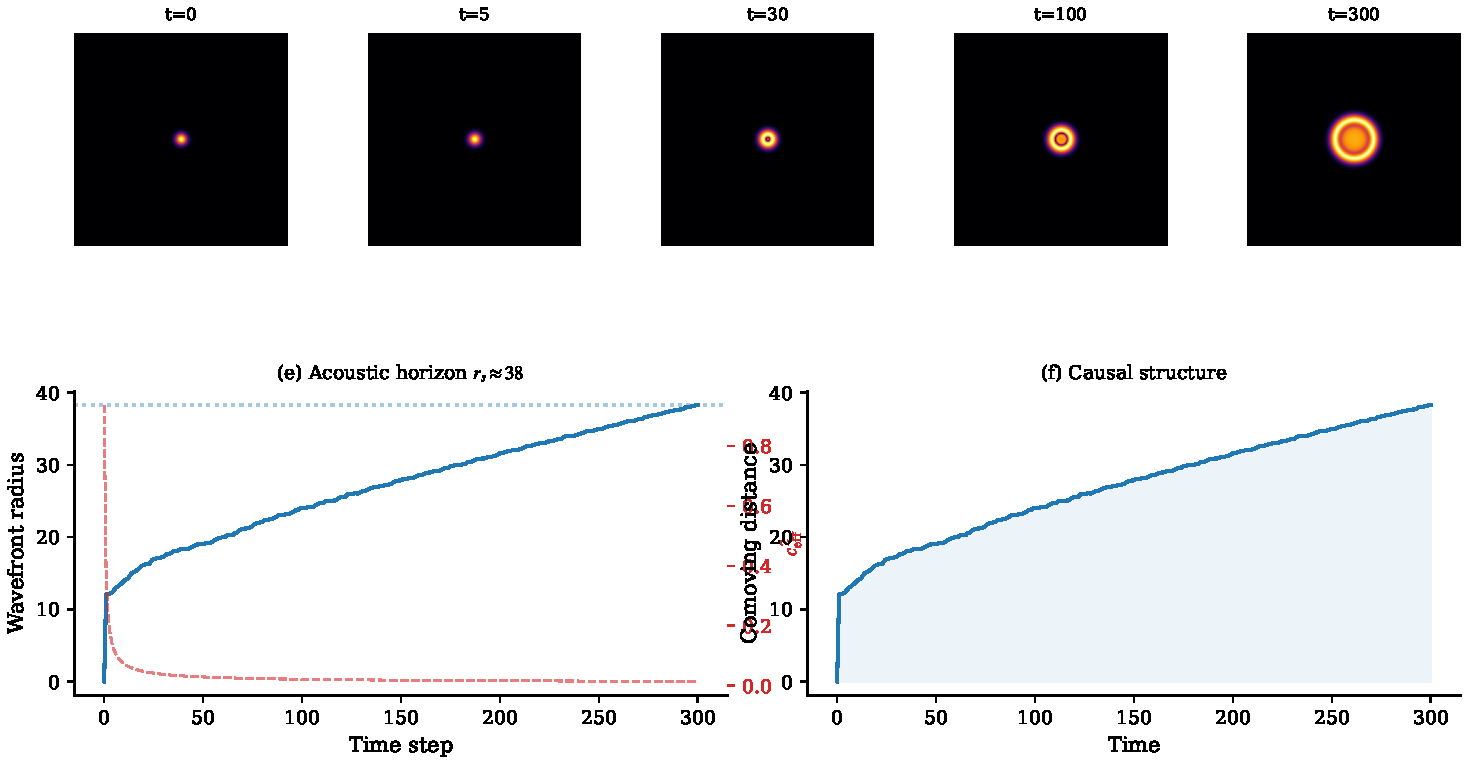
\includegraphics[width=\textwidth]{figures/fig5_freezeout.pdf}
    \caption{Acoustic freeze-out from $1/\ln^2(t)$ cooling.
    Top: wavefront snapshots at $t=0, 5, 30, 100, 300$.
    (e)~Wavefront radius (blue) saturates at $r_s \approx 38$; effective sound speed $c^2_{\rm eff}$ (red dashed) decays to zero.
    (f)~Causal structure showing the bending light cone produced by adiabatic cooling.}
    \label{fig:freezeout}
\end{figure*}

% Fig 6: Ensemble
\begin{figure}[t]
    \centering
    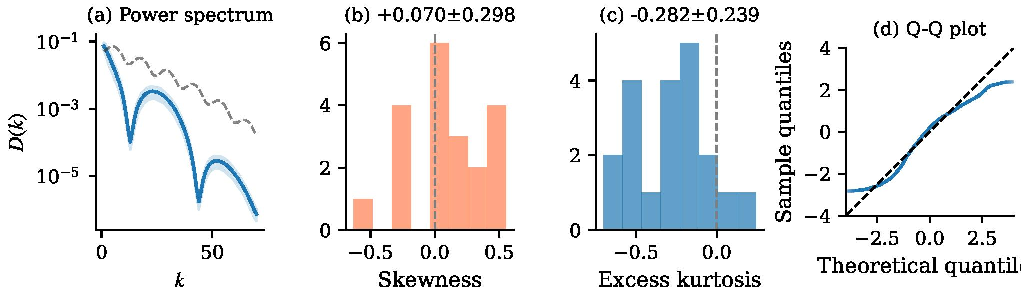
\includegraphics[width=\columnwidth]{figures/fig6_ensemble.pdf}
    \caption{Ensemble statistics from 20 independent DSC runs ($N=300$, 45 steps).
    (a)~Mean $D(k)$ with $\pm 1\sigma$ band and mock $\Lambda$CDM reference.
    (b,c)~Skewness and excess kurtosis distributions, both consistent with zero.
    (d)~Q-Q plot confirming near-Gaussian one-point statistics.}
    \label{fig:ensemble}
\end{figure}

% Fig 7: Sensitivity
\begin{figure*}[t]
    \centering
    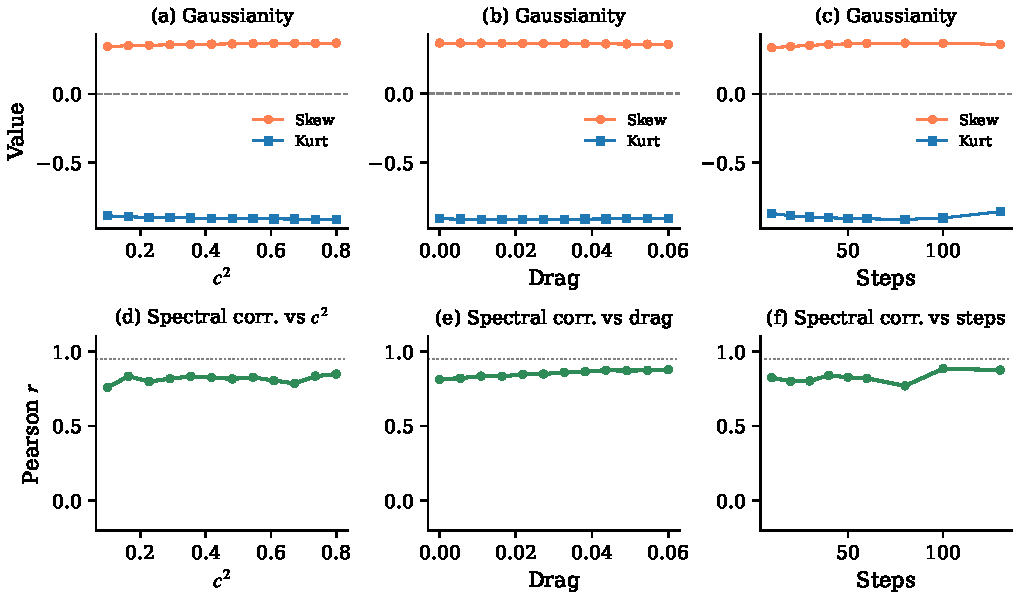
\includegraphics[width=\textwidth]{figures/fig7_sensitivity.pdf}
    \caption{Parameter sensitivity analysis.
    Top row: skewness (red) and excess kurtosis (blue) vs.\ $c^2$, drag, and evolution steps.
    Bottom row: Pearson spectral correlation with mock $\Lambda$CDM.
    Gaussianity and spectral shape are robust across wide parameter ranges.}
    \label{fig:sensitivity}
\end{figure*}

% Fig 8: Planck comparison
\begin{figure*}[t]
    \centering
    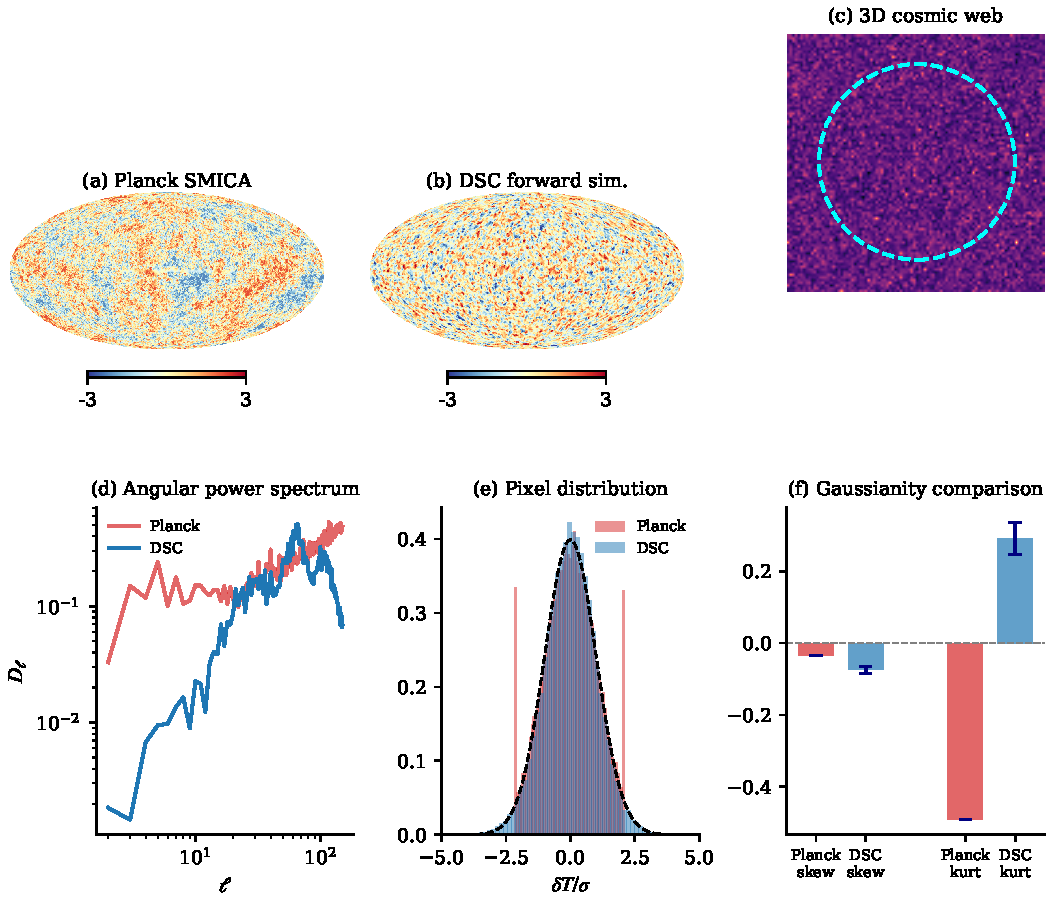
\includegraphics[width=\textwidth]{figures/fig8_planck_comparison.pdf}
    \caption{DSC 3D forward simulation vs.\ real Planck SMICA data.
    (a)~Planck SMICA full-sky map (Nside=64). (b)~DSC 3D $\to$ sphere projection.
    (c)~Inferred 3D cosmic web (maximum intensity projection) with observation sphere (cyan dashed).
    (d)~Angular power spectrum comparison. (e)~Pixel distributions. (f)~Gaussianity metrics with ensemble error bars.
    DSC skewness ($-0.075 \pm 0.009$) is close to Planck ($-0.036$); kurtosis sign differs ($+0.29$ vs.\ $-0.49$).}
    \label{fig:planck}
\end{figure*}
